\documentclass{article}

\usepackage{amssymb}
\usepackage{amsmath}
\usepackage[bottom]{footmisc}
\usepackage{bm}
\usepackage{caption}
\captionsetup[figure]{labelformat=empty, width=.5\paperwidth}

\usepackage{tikz}

\title{Summarising the \\ "Simpler Parametrized Algorithm for OCT" \\
\large by Daniel, Saket and Somnath}

\author{Florian Suess}
\date{}
\begin{document}
\maketitle
\section{Problem Introduction}
The odd cycle transversal problem on graph $G = (V, E)$ with integer $k$, denoted here as $OCT(G,k)$ is a predicate. True iff there exists an $S \subseteq V$ where $|S| \leq k$  st. $G' = (V \setminus S, E)$ contains no cycles of odd length. We say that $S$ is an odd cycle transversal (OCT) for $G$. 

Recall that a graph that doesn't contain odd-length cycles is bipartite, a very useful equivalence allowing us to use 2-colouring to drive intuition of the problem.

\begin{figure}[ht]
\centering
\begin{minipage}{0.45\textwidth}
\centering
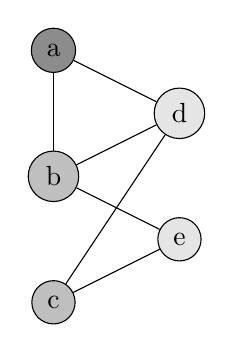
\begin{tikzpicture}[scale=0.8,every node/.style={draw,circle}]
    % nodes
    \node[fill=gray!90] (a) at (0,2) {a};
    \node[fill=gray!50] (b) at (0,0) {b};
    \node[fill=gray!50] (c) at (0,-2) {c};

    \node[fill=gray!20] (d) at (2,1) {d};
    \node[fill=gray!20] (e) at (2,-1) {e};

    % edges
    \draw (a) -- (d);
    \draw (a) -- (b);
    \draw (b) -- (d);
    \draw (b) -- (e);
    \draw (c) -- (d);
    \draw (c) -- (e);
\end{tikzpicture}
\end{minipage}\hfill
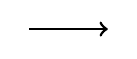
\begin{tikzpicture}
    \draw[->,line width=1pt] (0,0) -- (1,0);
\end{tikzpicture}\hfill
\begin{minipage}{0.45\textwidth}
\centering
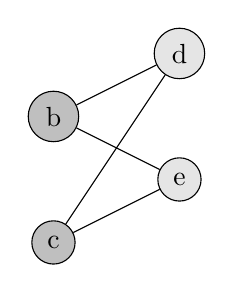
\begin{tikzpicture}[scale=0.8,every node/.style={draw,circle}]
    
    % Nodes
    \node[fill=gray!50] (b) at (0,0) {b};
    \node[fill=gray!50] (c) at (0,-2) {c};

    \node[fill=gray!20] (d) at (2,1) {d};
    \node[fill=gray!20] (e) at (2,-1) {e};

    % Edges
    \draw (b) -- (d);
    \draw (b) -- (e);
    \draw (c) -- (d);
    \draw (c) -- (e);

\end{tikzpicture}
\end{minipage}
\caption{$S = \{a\}$, notice $G' = (V \setminus S, E)$ is bipartite, $S$ is an OCT for this $G$.\protect\footnotemark}
\end{figure}
\footnotetext{Notice that we could also have $S=\{b\}$ or even $S=\{d\}$, OCT is not strictly unique!}

\section{Preliminaries}
We will arbitrarily order $V$ provided for $G$; $v_1v_2...v_n$, then let $V_i = \{v_1,v_2,...,v_i\}$ and denote $G[V_i]$ to be the subgraph induced over $V_i$.

For convenience we also like to have $G \setminus S$ = $G' = (V \setminus S, E)$.

\section{History}
This problem stems directly from the {\em looser} vertex deletion problem; finding the OCT $\bm{S}$ for $G$ such that for all other OCT's $S$ of $G$ we have $|\bm{S}| \leq |S|$. $S$ is colloquially known as a hitting set, peculiar name surfaces in conjunction to the other types of hitting sets;
\begin{itemize}
				\item Feedback Vertex Set (FVS): a vertex set that hits all cycles.
				\item Even Cycle Transversal (ECT): a vertex set that hits all cycles of even length.
\end{itemize}
Finding the minimal OCT of a graph $G$ is a well-known NP-Hard problem.

\subsection{Reed, Smith and Vetta}
The first significant results regarding an algorithm that demonstrated $OCT(G,k)$ is FPT was obtained in 2004 by Reed, Smith and Vetta\cite{reed-smith-vetta}. Their introduction of the iterative compression technique laid the groundwork for its use in various other parameterized algorithmic applications. The best resource I've found for describing this original algorithm has been published by the NPTEL collective\cite{nptel} but as Daniel, Saket and Somnath describe; this algorithm is known to be quite difficult to grasp, hence leading the motivation for this "simpler" approach.

\section{The Paper}
In simplest summary this paper defines a compressed version of this problem, call it $C(G', S', k)$ such that $G'$ is a subgraph of $G$, and $S'$ is an "almost" OCT set of $G'$, "almost" because $|S'| \leq k \bm{+ 1}$. This paper then shows why this problem is significantly simpler to solve, by defining an algorithm $C(G', S', k) \rightarrow S$ that returns a valid OCT for $G'$ {\em actively using} the information given from $S'$.\footnote{This summary on it's own is actually sufficient for both this paper's approach and the original Reed, Smith and Vetta's approach. Highlights how focal this iterative compression technique is.}

\pagebreak

\subsection{Algorithm Structure}
We summarise this paper into three significant parts;

\begin{enumerate}
	\item The iterative construction of bigger and bigger (wrt. size of subgraph $G'$) compressed versions of the OCT problem, eventually coinciding with the subgraph $G' = G$.
	\item The bounded iteration of possible solution spaces for the compressed problem highlighting the $f(k)$ part of the FPT algorithm.
	\item An algorithm that linearly determines if the solution space provided above contains an OCT for the compressed problem.   
\end{enumerate}

Naturally in terms of algorithmic structure you then have this "outer loop", "middle loop" and "inner loop". We only provide commentary for the first two here, and unfortunately leave the reader to continue studying the "inner loop".

\subsubsection{Outer Loop: Construction of compressed OCT problems}
We have the following two very simple observations.\footnote{Paper mentions another observation here; assuming $G$ has a valid OCT $S$, then $S \cap V_i$ is an OCT of $G[V_i]$ for $i \leq n$, though I found it irrelevant.}

\begin{itemize}
				\item $V_k$ is an OCT of $G[V_k]$.
				\item If $S$ is an OCT of $G[V_i]$, then $S \cup \{v_{i+1}\}$ is an OCT of $G[V_{i+1}]$.
\end{itemize}

The first observation is used as a way to kick start that outer loop with compressed problem $C(G[V_{k+1}], V_{k+1}, k)$. We assume for any $i$ that $C(G[V_i], S', k) \rightarrow S$ (next two sections). Given the previous iteration yields a valid OCT $S$ for $G[V_i]$, we can iteratively construct a larger compressed problem via; 

\begin{align*}
C(G[V_i] \cup \{v_{i+1}\}, S \cup \{v_{i+1}\}, k)
\end{align*}
\\~\\
This happens {\em less than} $|V|$ times (precisely at most $|V| - k$).

\subsubsection{Middle Loop: Iterating all solution spaces via the "close" OCT}
Zooming into the $C(G, S', k) \rightarrow S$ mapping now\footnote{We originally introduced this with $G[V_i]$, but changing this to $G$ here to simplify for readability.}. The authors draw us to the realisation that {\em if} indeed there exists an OCT $S$ with size $\leq k$ for $G$, then there must exist a partitioning of $S'$ itself into $L, R$ and $T$ such that $L$ and $R$ are subsets themselves of the bigger partitioning that would happen on this given $G$ if for some other set $T'$ (which we will later find) we have a valid resulting bipartite graph $G \setminus T \cap T'$ (where of course $T \cap T' = S$ and $T \cap T' \leq k$).
\\~\\
Hence we iterate through {\em at most} $3^k$ partitions of $S'$ (since $|S'| \leq k + 1$).

\subsubsection{Inner Loop: Attempt to construct an OCT}
Obviously skipping all partitions of $S'$ where $G[L]$ or $G[R]$ contains any edges as these need to represent the subsets of partitions of a bipartite graph. We now leave it to you to learn about how we use $S'$ to construct a $T'$, and use auxiliary vertices $s$, $t$ to run a max-flow algorithm $O(k \cdot |E|)$ on to check whether the found $T' \cap T$ is a valid OCT for $G$.

\subsection{Algorithm Complexity}
Simply stitching the three parts together.
\begin{align*}
O(|V| \cdot 3^k \cdot k \cdot |E|) = O (f(k) \cdot n^{O(1)})
\end{align*}

\begin{thebibliography}{9}
\bibitem{reed-smith-vetta}
B. Reed, K. Smith and A. Vetta, "Finding Odd Cycle Transversals", Operations Research Letters, 32, 229–301 (2004).
\bibitem{nptel}
National Programme of Technologically Enhanced Learning, "Parameterized Algorithms" Module 3, Lecture 15, youtube.com/watch?v=oaOUXiSo2xg (2022).
\bibitem{daniel-saket-somnath}
D. Lokshtanov, S. Saurabh, S. Sikdar, "Simpler Parameterized Algorithm for OCT", Attached (2009).
\end{thebibliography}
\end{document}
